\section{The Standard Model of Particle Physics}

The standard model (SM) of particle physics describes all of the known
particles and their interactions through the fundamental forces
(except for gravity): the strong nuclear force, the weak nuclear force, and the electromagnetic
force. These forces arise due to the exchange of spin-$1$
bosons among the spin-$\frac{1}{2}$ fermions that make up matter. The SM is a renormalizable quantum field
theory based on the gauge symmetry group $\mathrm{SU(3)}_{\mathrm{C}}\times \mathrm{SU(2)}_{\mathrm{L}}\times
\mathrm{U(1)}_Y$. Each factor in the gauge group corresponds to a fundamental force, represented by a gauge field, whose excitations are
the gauge bosons that act as force carriers:
\begin{center}
\begin{tabular}{ccccc}
$\mathrm{SU(3)}_{\mathrm{C}}$ &$\times$& $\mathrm{SU(2)}_{\mathrm{L}}$
  &$\times$& $\mathrm{U(1)}_Y$\\
 $\downarrow$&&$\downarrow$&&$\downarrow$\\
 $G_{\mu}^{\alpha}$&&$W^a_{\mu}$&&$B_{\mu}$\\
 $\alpha=1,...,8$&&$a=1,2,3$&&
\end{tabular}
\end{center}
The eight spin-$1$ bosons, $G_{\mu}^{\alpha}$,
associated with the factor $\mathrm{SU(3)}_{\mathrm{C}}$ are the gluons. Any
particle that transforms is said to carry color charge. The three spin-$1$
bosons, $W^{a}_{\mu}$ are associated 

The matter fields are fermions, which fall into two
categories: the quarks, $u$, $d$, $c$, $s$, $t$, and $b$, which participate in the
strong interactions, and the leptons, $e$, $\mu$, $\tau$, $\nu_e$,
$\nu_{\mu}$, and $\nu_{\tau}$, which do
not. Fig.~\ref{fig:standardmodel} shows the particles in the SM. To simplify notation, it makes sense to consider the doublet of
$q_L = \binom{u_L}{d_L}$ and $\ell_L = \binom{e_L}{\nu_L}$. All matter fields implicity have
three-component generation indices $e_i=(e,\mu,\tau),
\nu_i=(\nu_e,\nu_{\mu},\nu_{\tau}), u_i=(u,c,t),
d_i=(d,s,b)$. 

The electric charge is given by $Q = T_{3L}+Y$. Tab.~\ref{tab:representations} summarizes the
representations in which the fields transform under the SM
gauge group. The SM Langrangian
excluding Higgs and Yukawa terms is then,
\begin{align}
\mathcal{L}_{\mathrm{SM}} &= -\frac{1}{4}B_{\mu\nu}B^{\mu\nu} -\frac{1}{4}W^{a}_{\mu\nu}W^{a\mu\nu} - \frac{1}{4}G^{\alpha}_{\mu\nu}G^{\alpha\mu\nu}
  & \mathrm{(gauge~terms)}\nonumber\\
& +\bar\ell_L\tilde\sigma^{\mu}iD_{\mu}\ell_L +
   \bar e_R\sigma^{\mu}iD_{\mu}e_R + \bar v_R
   \sigma^{\mu}iD_{\mu}\nu_R + (\mathrm{h.c.})& \mathrm{(lepton~kinetic~terms)}\nonumber\\
& +\bar q_L\tilde\sigma^{\mu}iD_{\mu}q_L +
   \bar u_R\sigma^{\mu}iD_{\mu}u_R + \bar d_R
   \sigma^{\mu}iD_{\mu}d_R + (\mathrm{h.c.})& \mathrm{(quark~kinetic~terms)}\nonumber\\
& +\mathcal L_{\mathrm{Higgs}} +\mathcal L_{\mathrm{Yukawa}} &  \mathrm{(Higgs~and~Yukawa~terms)}
\label{eqn:lsm}
\end{align}
where $D_{\mu}$ is the gauge covariant derivative.

\begin{figure}
\centering
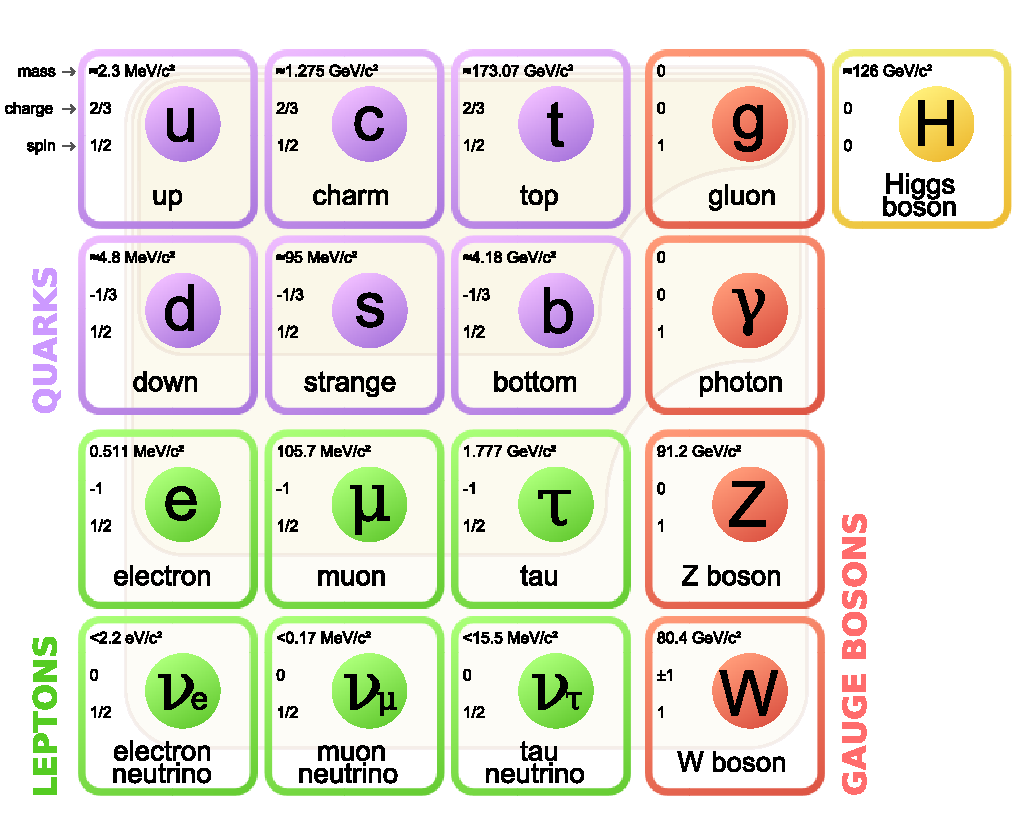
\includegraphics[width=0.7\textwidth]{figs/theory/standardmodel.pdf}
\caption{\label{fig:standardmodel} The particles in the standard model.}
\end{figure}

\begin{table}
\centering
\begin{tabular}{c|ccc}
&$\mathrm{SU(3)}_{\mathrm{C}}$&$\mathrm{SU(2)}_{\mathrm{L}}$&$\mathrm{U(1)}_Y$ \\
$q$ & $\mathbf{3}$ & $\mathbf{2}$ & $1/6$\\
$\bar u_R$ & $\mathbf{\bar 3}$ & $\mathbf{1}$ & $-2/3$\\
$\bar d_R$ & $\mathbf{\bar 3}$ & $\mathbf{1}$ & $1/3$\\
$\ell$ & $\mathbf{1}$ & $\mathbf{2}$ & $-1/2$\\
$\bar e_R$ & $\mathbf{1}$ & $\mathbf{1}$ & $1$\\\hline
$h$ & $\mathbf{1}$ & $\mathbf{2}$ & $1/2$
\end{tabular}
\caption{\label{tab:representations} Table summarizing the
    representations in which the fields transform under the standard
    model gauge group.}
\end{table}


\section{Electroweak Symmetry Breaking}
A central feature of gauge theories is that the gauge bosons are
massless due to the fact that the gauge symmetry forbids explicit mass
terms in the Lagrangian. In 1964, it was proposed that spontaneous symmetry breaking in gauge
theories could be achieved through the introduction of a scalar
field~\cite{PhysRevLett.13.321,HIGGS1964132,PhysRevLett.13.508,PhysRevLett.13.585,PhysRev.145.1156,PhysRev.155.1554}. In
the SM, the mechanism of electroweak symmetry breaking
is a framework to keep the structure of gauge symmetry and
interactions at high energy, and still generate the observed masses
of the $\PW$ and $\PZ$ gauge
bosons~\cite{PhysRevLett.19.1264,GLASHOW1961579,Salam:1968rm}. The SM
Higgs part of the Lagrangian is: 
\begin{align}
\mathcal L_{\mathrm{Higgs}} &= (D_{\mu}\Phi)^{\dagger}(D^{\mu}\Phi) -
V(\Phi)~;& V(\Phi) &= -\mu^2\Phi^{\dagger}\Phi +
\lambda(\Phi^{\dagger}\Phi)^2~,
\label{eqn:Lhiggs}
\end{align}
where the field $\Phi$ is a self-interacting
$\mathrm{SU(2)}_{\mathrm{L}}$ complex doublet with weak hypercharge $Y=1/2$:
\begin{equation}
\Phi = \left(\begin{matrix} \phi^{+}\\\phi^0\end{matrix} \right)~.
\end{equation}
If the quadratic term is negative, that is $\mu^2>0$, then the
potential will have a ``Mexican hat'' shape, illustrated in
\ref{fig:mexicanhat}, and the minimum of the potential will occur at a value of the field that is not $\mathrm{SU(2)}_{\mathrm{L}}\times\mathrm{U(1)}_Y$
invariant. Due to this, the complex scalar doublet field acquires a nonzero vacuum
expectation value (\emph{vev}), corresponding to the minimum of the potential,
\begin{align}
\langle\Phi\rangle_0&\equiv \langle 0|\Phi|0\rangle =
\frac{1}{\sqrt{2}}U(x)\left(\begin{matrix} 0\\v\end{matrix} \right)~;&v &= \sqrt{\frac{\mu^2}{\lambda}};
\end{align}
where $U(x)$ is a unitary transformation that rotates the field
to the other degenerate solutions. Since the vev is still symmetric under a $\mathrm{U(1)}$ subgroup of the full
electroweak symmetry, we say the electroweak symmetry
$\mathrm{SU(2)}_{\mathrm{L}}\times\mathrm{U(1)}_Y$ is \emph{spontaneously
broken} to $\mathrm{U(1)}_{\mathrm{EM}}$. Spontaneous symmetry breaking
is the phenomenon in which the equations of the dynamics are
exactly symmetric, but they admit solutions that are not.

\begin{figure}
\centering
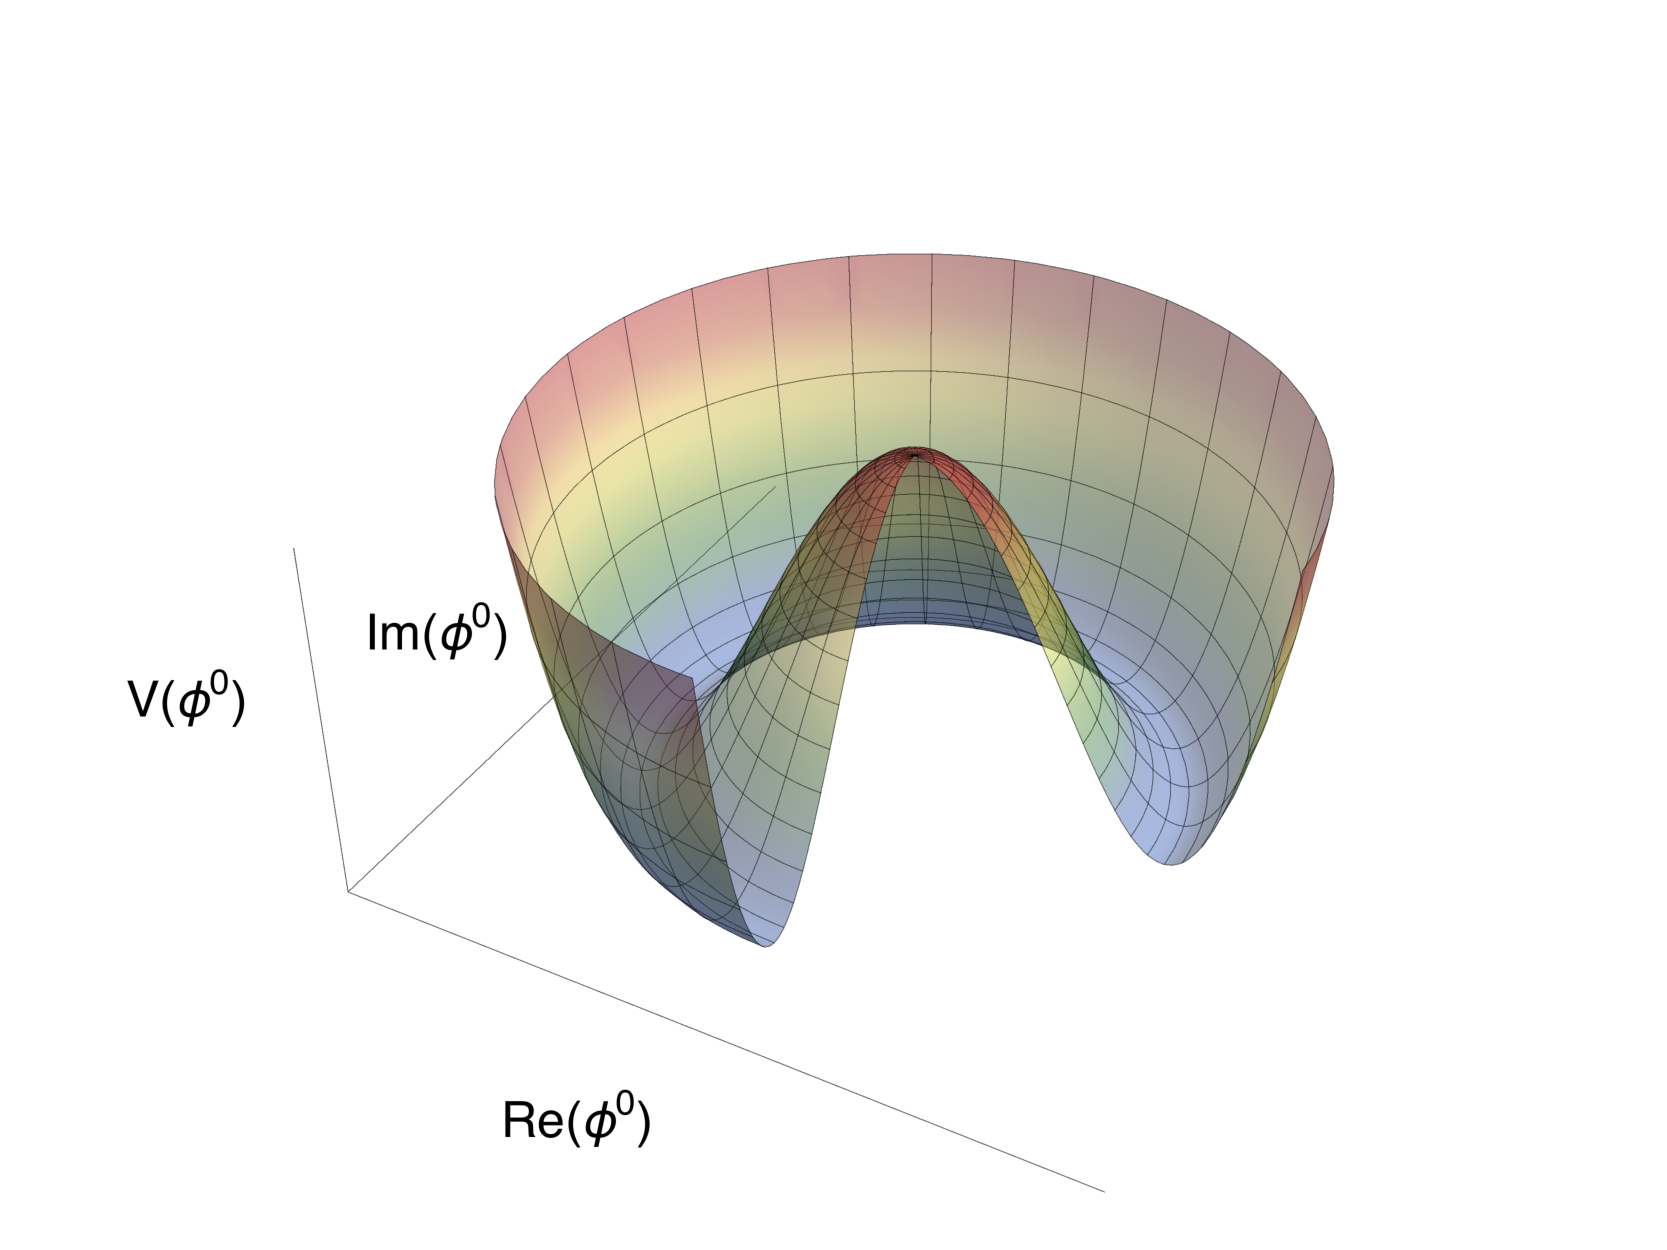
\includegraphics[width=0.7\textwidth]{figs/theory/MexicanHat.pdf}
\caption{\label{fig:mexicanhat} The shape of the ``mexican hat''
  potential. The minimum of the potential occurs at
a field value that is not 0.}
\end{figure}

This mechanism is responsible for generating the masses of the gauge
bosons in the standard model, as can be seen by evaluating the 
covariant derivative in Eqn.~\ref{eqn:Lhiggs},
\begin{equation}
D_{\mu}\Phi = (\partial_{\mu} - i g_2 \frac{\sigma_a}{2}W^a_{\mu} -
ig_1\frac{1}{2}B_{\mu})\Phi ~,
\end{equation}
on the vacuum Higgs field. In this case, the kinetic term is:
\begin{align}
|D_{\mu}\Phi|^2 &= \frac{1}{2} \left|\left (\begin{matrix}\partial_{\mu}
    -\frac{i}{2}(g_2W_{\mu}^3 + g_1B_{\mu})&
    -\frac{ig_2}{2}(W_{\mu}^1-iW_{\mu}^2)\\ 
-\frac{ig_2}{2}(W_{\mu}^1+iW^2_{\mu})&\partial_{\mu}
    +\frac{i}{2}(g_2W_{\mu}^3 - g_1B_{\mu})
  \end{matrix}\right)
                                       \left(\begin{matrix}0\\v\end{matrix}\right)\right |^2 \nonumber\\
& = \frac{1}{8} \left ( g_2^2v^2|W_{\mu}^1+iW^2_{\mu}|^2 +
  v^2|g_2W^3_{\mu}-g_1B_{\mu}|^2 \right ) \nonumber\\
& = m_W^2W_{\mu}^+W^{-\mu} +
\frac{1}{2}m_Z^2Z_{\mu}Z^{\mu}~ + \frac{1}{2}m_{\gamma}^2A_{\mu}A^{\mu},
\end{align}
where we can identify three field combinations, $W_{\mu}^{\pm}$ and
$Z_{\mu}$, which have bilinear mass terms, and a fourth $A_{\mu}$,
which does not:
\begin{align}
W_{\mu}^{\pm} &= \frac{1}{\sqrt{2}}(W_{\mu}^1\mp iW^2_{\mu})~, &m_W &= \frac{1}{2}vg_2~,\\
Z_{\mu} &= \frac{g_2W_{\mu}^3 - g_1B_{\mu}}{\sqrt{g_1^2+g_2^2}}~,&m_Z &= \frac{1}{2}v\sqrt{g_1^2+g_1^2}~,\\
A_{\mu} &= \frac{g_2W_{\mu}^3 + g_1B_{\mu}}{\sqrt{g_1^2+g_2^2}}~,&m_{\gamma} &= 0.
\end{align}
The $\PW$ and $\PZ$ bosons have acquired mass, while the photon
$\Pgg$ remains massless.

Another consequence of this symmetry breaking mechanism is the
emergence of a physical scalar boson. If we expand the field around
its potential minimum
\begin{align}
\Phi(x)&=
\frac{1}{\sqrt{2}}U(x)\left(\begin{matrix} 0\\v+H(x)\end{matrix} \right)
\end{align}
and write out the terms associated to this field, we find
\begin{equation}
\mathcal L_{\mathrm{Higgs}} \supset \frac{1}{2}(\partial^{\mu}H)^2 -
\lambda v^2 H^2 - \lambda v H^3 - \frac{\lambda}{4}H^4~.
\end{equation}
which means this scalar boson, called the \emph{Higgs boson}, is self-interacting and has a mass squared of $m^2_{h^0} =
2\lambda v^2$ at tree-level.

\subsection{Fermion Masses}
As proposed by Weinberg~\cite{PhysRevLett.19.1264}, fermions acquire
mass through interaction with the $\Phi$ field, which has a nonzero
vev. This is accomplished by adding Yukawa terms to the Lagrangian for
each generation,
\begin{equation}
\mathcal L_{\mathrm{Yukawa}} = - \lambda_e \bar\ell_L\Phi e_R -
\lambda_u\bar q_L\Phi u_R  - \lambda_d\bar q_L\tilde\Phi d_R + (\mathrm{h.c.})~,
\end{equation}
where the doublet $\tilde\Phi = i\sigma_2\Phi^{\ast}$ with hypercharge $Y=-1/2$ is
needed to generate masses for the down-type quarks. Then we can
identify the fermion masses as
\begin{align}
m_e &= \frac{\lambda_e v}{2}&m_u &= \frac{\lambda_e
                                          v}{2}& m_d &= \frac{\lambda_dv}{2}~.
\end{align}
Neutrino masses can also be accommodated in the SM by adding similar terms.


\section{Higgs Mass and Naturalness}
The leading quantum correction to the Higgs mass squared parameter is due to
the large Yukawa coupling coupling to the top quark, which gives the
top quark its large mass,
\begin{fmffile}{higgs}
\begin{align}
\Delta(m^2_{h^0}) &= \quad\parbox{20mm}{
\begin{fmfgraph*}(20,20)
\fmfkeep{fermion}
\fmfleft{i} 
\fmfright{o} 
\fmf{dashes}{i,v1}
\fmf{dashes}{v2,o}
\fmf{plain,left,tension=.3,label=$t$}{v1,v2}
\fmf{plain,left,tension=.3}{v2,v1}
\fmfv{label=$h^0$,label.angle=90}{i}
\end{fmfgraph*}} \quad + \quad\cdots\\
&= -\frac{|\lambda_t|^2}{8\pi^2}\Lambda_{\mathrm{UV}}^2 + \cdots~,
\end{align}
where $\Lambda_{\mathrm{UV}}$ is an ultraviolet momentum cutoff.

\begin{align}
\Delta(m^2_{h^0}) &= \quad\parbox{20mm}{\fmfreuse{fermion}} \quad + \quad
\parbox{20mm}{
\begin{fmfgraph*}(20,20)
\fmfkeep{boson}
\fmfleft{i} 
\fmfright{o} 
\fmf{dashes}{i,v}
\fmf{dashes,right,tension=0.7,label=$\tilde t_{1,,2}$}{v,v}
\fmf{dashes}{v,o}
\fmfv{label=$h^0$,label.angle=90}{i}
\end{fmfgraph*}}
 \quad + \quad
\parbox{20mm}{
\begin{fmfgraph*}(20,20)
\fmfkeep{sunset}
\fmfleft{i}
\fmfright{o}
\fmf{dashes}{i,v1}
\fmf{dashes}{v2,o}
\fmf{dashes,left,tension=.3,label=$\tilde t_{1,,2}$}{v1,v2}
\fmf{dashes,left,tension=.3}{v2,v1}
\fmfv{label=$h^0$,label.angle=90}{i}
\end{fmfgraph*}} \quad + \quad\cdots\\
 &= -\frac{|\lambda_t|^2}{8\pi^2}\Lambda_{\mathrm{UV}}^2 +
  \sum_{i=1}^{2} \left ( \frac{\lambda_{\tilde
  t_i}^2}{16\pi^2}\Lambda_{\mathrm{UV}}^2 - 2m_{\tilde
  t_i}^2\log(\Lambda_{\mathrm{UV}}/m_{\tilde t_i}) \right )+ \cdots~,
\end{align}
\end{fmffile}

\section{Supersymmetry}
Supersymmetry (SUSY) is a proposed symmetry of spacetime that 
introduces a bosonic (fermionic) partner for every fermion (boson) in the 
standard model
(SM)~\cite{Wess,Golfand,Volkov,Chamseddine,Kane,Fayet,Barbieri,Hall,Ramond}.

Supersymmetric extensions of the SM are particularly compelling 
because they yield solutions to the gauge hierarchy problem with no
fine-tuning of fundamental parameters~\cite{Witten:1981nf,Dimopoulos:1981zb,Dine:1981za,Dimopoulos:1981au,Sakai:1981gr,Kaul:1981hi}, 
exhibit gauge coupling unification~\cite{Dimopoulos:1981yj,Marciano:1981un,Einhorn:1981sx,Ibanez:1981yh,Amaldi:1991cn,Langacker:1995fk},
and provide weakly interacting particle candidates for dark matter~\cite{Ellis:1983ew,Jungman:1995df}.
For SUSY to provide a ``natural'' solution to the gauge hierarchy problem,
the top squark, bottom squark, and gluino must have masses below a few
TeV, making them accessible at the CERN LHC. 

An operator $Q$ that generates supersymmetry transformations is an
anti-commuting spinor with
\begin{equation}
Q|\mathrm{boson}\rangle = |\mathrm{fermion}\rangle, ~~~~
Q|\mathrm{fermion}\rangle = |\mathrm{boson}\rangle~.
\end{equation}

The group of symmetries of spacetime in four-dimensional quantum field
theory is known as the Poincar\'{e} group. The generators of the
Poincar\'{e} group consist of the energy-momentum vector $P_m$ and the
Loretnz generators $M_{mn} = -M_{nm}$. The Poincar\'{e} algebra is
\begin{align}
~[P_m,P_n] &= 0 \nonumber\\
~[P_m,M_{np}] &= i(\eta_{mn}P_p-\eta_{mp}P_n) \nonumber\\
~[M_{mm},M_{pq}] &= i(\eta_{mp}M_{np} - \eta_{np}M_{mq} +
                   \eta_{nq}M_{mp} - \eta_{mq}M_{np} )~.
\label{eqn:poincare}
\end{align}

As shown by Coleman and Mandula~\cite{PhysRev.159.1251}, every local renormalizable quantum
field theory in four-dimensional Minkowski spacetime with that
satisfies a simple set of three assumptions (finite number of different
one-particle states, non-trivial interactions, and a mass gap) can only have a symmetry \emph{Lie algebra} of the S matrix which is a
direct product of the Poincar\'{e} group and an internal symmetry group $G$:
$($Poincar\'{e}$)\times G$. In other words, spacetime and
internal symmetries may only be combined in a trivial way. More explicitly, if $G$ has a Lie algebra $\mathcal
G$ of the form
\begin{equation}
~[B_r,B_s] = f_{rs}{}^tB_t~,
\end{equation}
where $f_{rs}{}^t$ are structure functions, then the Coleman-Mandula theorem implies that
\begin{equation}
~[B_r,P_m] = [B_r,M_{mn}] = 0~.
\end{equation}

However, the CM theorem has a loophole in that it assumes the
symmetry algebra of the $S$ matrix contains only \emph{commutation
relations}. In fact, it is possible to generalize the idea of a symmetry algebra to include
fermionic charges with \emph{anticommutation relations} in addition to the
usual bosonic charges with commutation relations. 

With this generalization, there is a non-trivial way to combine
supersymmetry transformation generator $Q$ with the Poincar\'{e} group
in a way that mixes the two
symmetry. The simplest example is given by the super Lie algebra for $\mathcal N=1$
supersymmetry,
\begin{align}
~\{ Q_{\alpha},\bar Q_{\dot{\beta}}\} &= 2\sigma^m_{\alpha\dot\beta} P_m \nonumber\\
~\{ Q_{\alpha},Q_{\beta}\} &= \{ \bar Q_{\dot\alpha},\bar Q_{\dot\beta}\} = 0\nonumber\\
~[ P_m, Q_{\alpha}] &= [P_m,\bar Q_{\dot\alpha}] = 0~.
\label{eqn:n1susy}
\end{align}

The simplest supersymmetric extension of the standard model is the
Minimal Supersymmetric Standard Model (MSSM). 
The K\"{a}hler potential and super potential for chiral superfields
\begin{equation}
\mathcal L = \int \mathrm{d}^4\theta K(\Phi,\Phi^{\dagger}) + \left (\int
 \mathrm{d}^2\theta W(\Phi) + \mathrm{h.c.} \right)
\label{eqn:mssmlag}
\end{equation}

\begin{table}
\centering
\begin{tabular}{c|ccc}
&$\mathrm{SU(3)}_{\mathrm{C}}$&$\mathrm{SU(2)}_{\mathrm{L}}$&$\mathrm{U(1)}_Y$ \\
$Q$ & $\mathbf{3}$ & $\mathbf{2}$ & $1/6$\\
$U^c$ & $\mathbf{\bar 3}$ & $\mathbf{1}$ & $-2/3$\\
$D^c$ & $\mathbf{\bar 3}$ & $\mathbf{1}$ & $1/3$\\
$L$ & $\mathbf{1}$ & $\mathbf{2}$ & $-1/2$\\
$E^c$ & $\mathbf{1}$ & $\mathbf{1}$ & $1$\\\hline
$H_u$ & $\mathbf{1}$ & $\mathbf{2}$ & $1/2$\\
$H_d$ & $\mathbf{1}$ & $\mathbf{2}$ & $-1/2$
\end{tabular}
\caption{\label{tab:representations} Table summarizing the
    representations in which the superfields transform under the standard
    model gauge group.}
\end{table}

The R-parity conserving part of the superpotential is whown in Eqn.~\ref{eqn:Wrpc}
\begin{equation}
W_{\mathrm{RPC}} = - y_u H_u Q U^c + y_dH_d Q D^c + y_e H_d L E^c +
\mu H_uH_d
\label{eqn:Wrpc}
\end{equation}
while the R-partiy violating part is shown in \ref{eqn:Wrpv}
\begin{equation}
W_{\mathrm{RPV}} =\frac{1}{2}\lambda^{ijk}L_iL_jE_k^c +
\lambda^{\prime ijk} L_iQ_jD_k^c + \mu^{\prime i}H_uL_i +
\frac{1}{2}\lambda^{\prime\prime ijk}U_i^cD_j^cD_k^c
\label{eqn:Wrpv}
\end{equation}
From this we can write down the Lagrangian for the MSSM
\begin{equation}
\mathcal L_{\mathrm{MSSM}}=\frac{1}{2}\lambda^{ijk}L_iL_jE_k^c +
\lambda^{\prime ijk} L_iQ_jD_k^c + \mu^{\prime i}H_uL_i +
\frac{1}{2}\lambda^{\prime\prime ijk}U_i^cD_j^cD_k^c
\label{eqn:Wrpv}
\end{equation}

The mass matrices for the neutralinos and charginos are given by
\begin{equation}
\mathbf{M}_N =\left (  \begin{matrix}
M_1 & 0 & -m_Zs_Wc_{\beta} & m_Zs_Ws_{\beta} \\
0& M_2 & -m_Zc_Wc_{\beta} & -m_Zc_Ws_{\beta} \\
-m_Zs_Wc_{\beta}& m_zc_Wc_{\beta} & 0 & -\mu\\
m_Zs_Ws_{\beta}& -m_zc_Ws_{\beta} & \mu & 0
\end{matrix}\right)~,
\end{equation}
and 
\begin{equation}
\mathbf{M}_C =\left (  \begin{matrix}
M_2 & \sqrt{2}m_Ws_{\beta}\\
 \sqrt{2}m_Wc_{\beta}& \mu
\end{matrix}\right)~,
\end{equation}
respectively. When the lightest neutralino is Higgsino-like ($\mu \ll M_1, M_2$), the
mass eigenvalues of the lightest neutralino, second lightest neutralino and chargino are close to
each other,
\begin{align}
m_{\chiz_1} &= \mu + \frac{m_Z^2(1+s_{\beta})(\mu - M_1c_W^2-M_2s_W^2)}{2(\mu-M_1)(\mu-M_2)} + \cdots\\
m_{\chiz_2} &= \mu + \frac{m_Z^2(1-s_{\beta})(\mu + M_1c_W^2+M_2s_W^2)}{2(\mu+M_1)(\mu+M_2)} + \cdots\\
m_{\chipm_1} &= \mu - \frac{m_W^2(\mu + M_2\sin 2\beta)}{M_2^2-\mu^2} + \cdots
\end{align}

Fig.~\ref{fig:neutralinos} shows the mass differences
$m_{\chipm_1}-m_{\chiz_1}$ and $m_{\chiz_2}-m_{\chiz_1}$ as a function of the Wino mass $M_2$.


\begin{figure}[tb!]
\centering
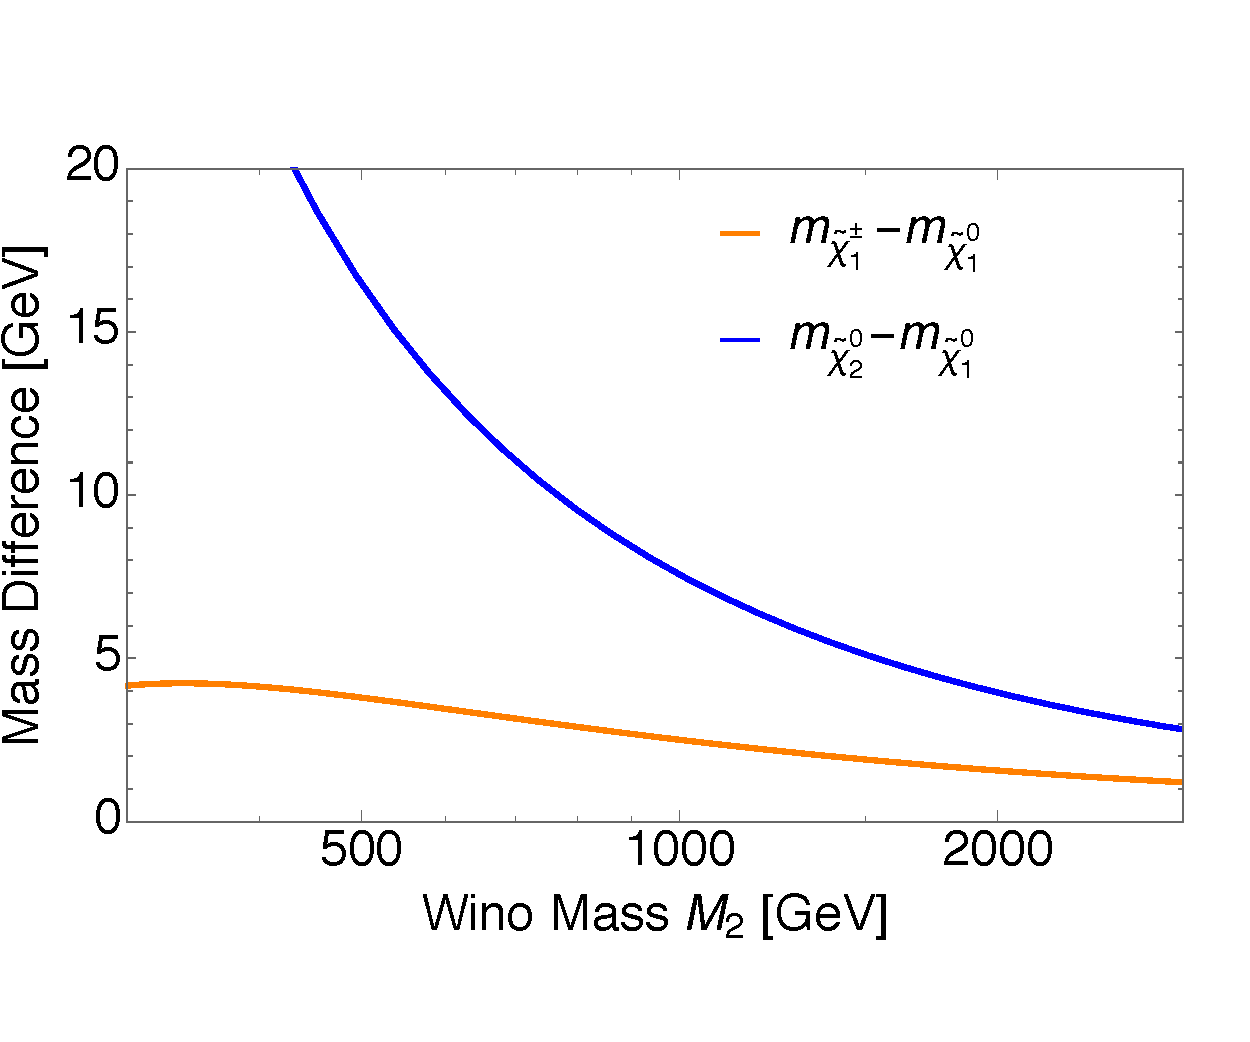
\includegraphics[width=0.8\textwidth,clip=true,viewport= 0 30 610 450]{figs/theory/neutralinos.pdf}
\caption{The mass difference between the lightest chargino and the
  lightest neutralino as a function of the Wino mass $M_2$
  assuming $\tan\beta=10$, $\mu=200 \GeV$ and $M_1 = 3 \TeV$.\label{fig:neutralinos}}
\end{figure}

\section{Simplified Natural Supersymmetry Models}
\label{sec:sms}

\begin{figure}[htb!]
\centering
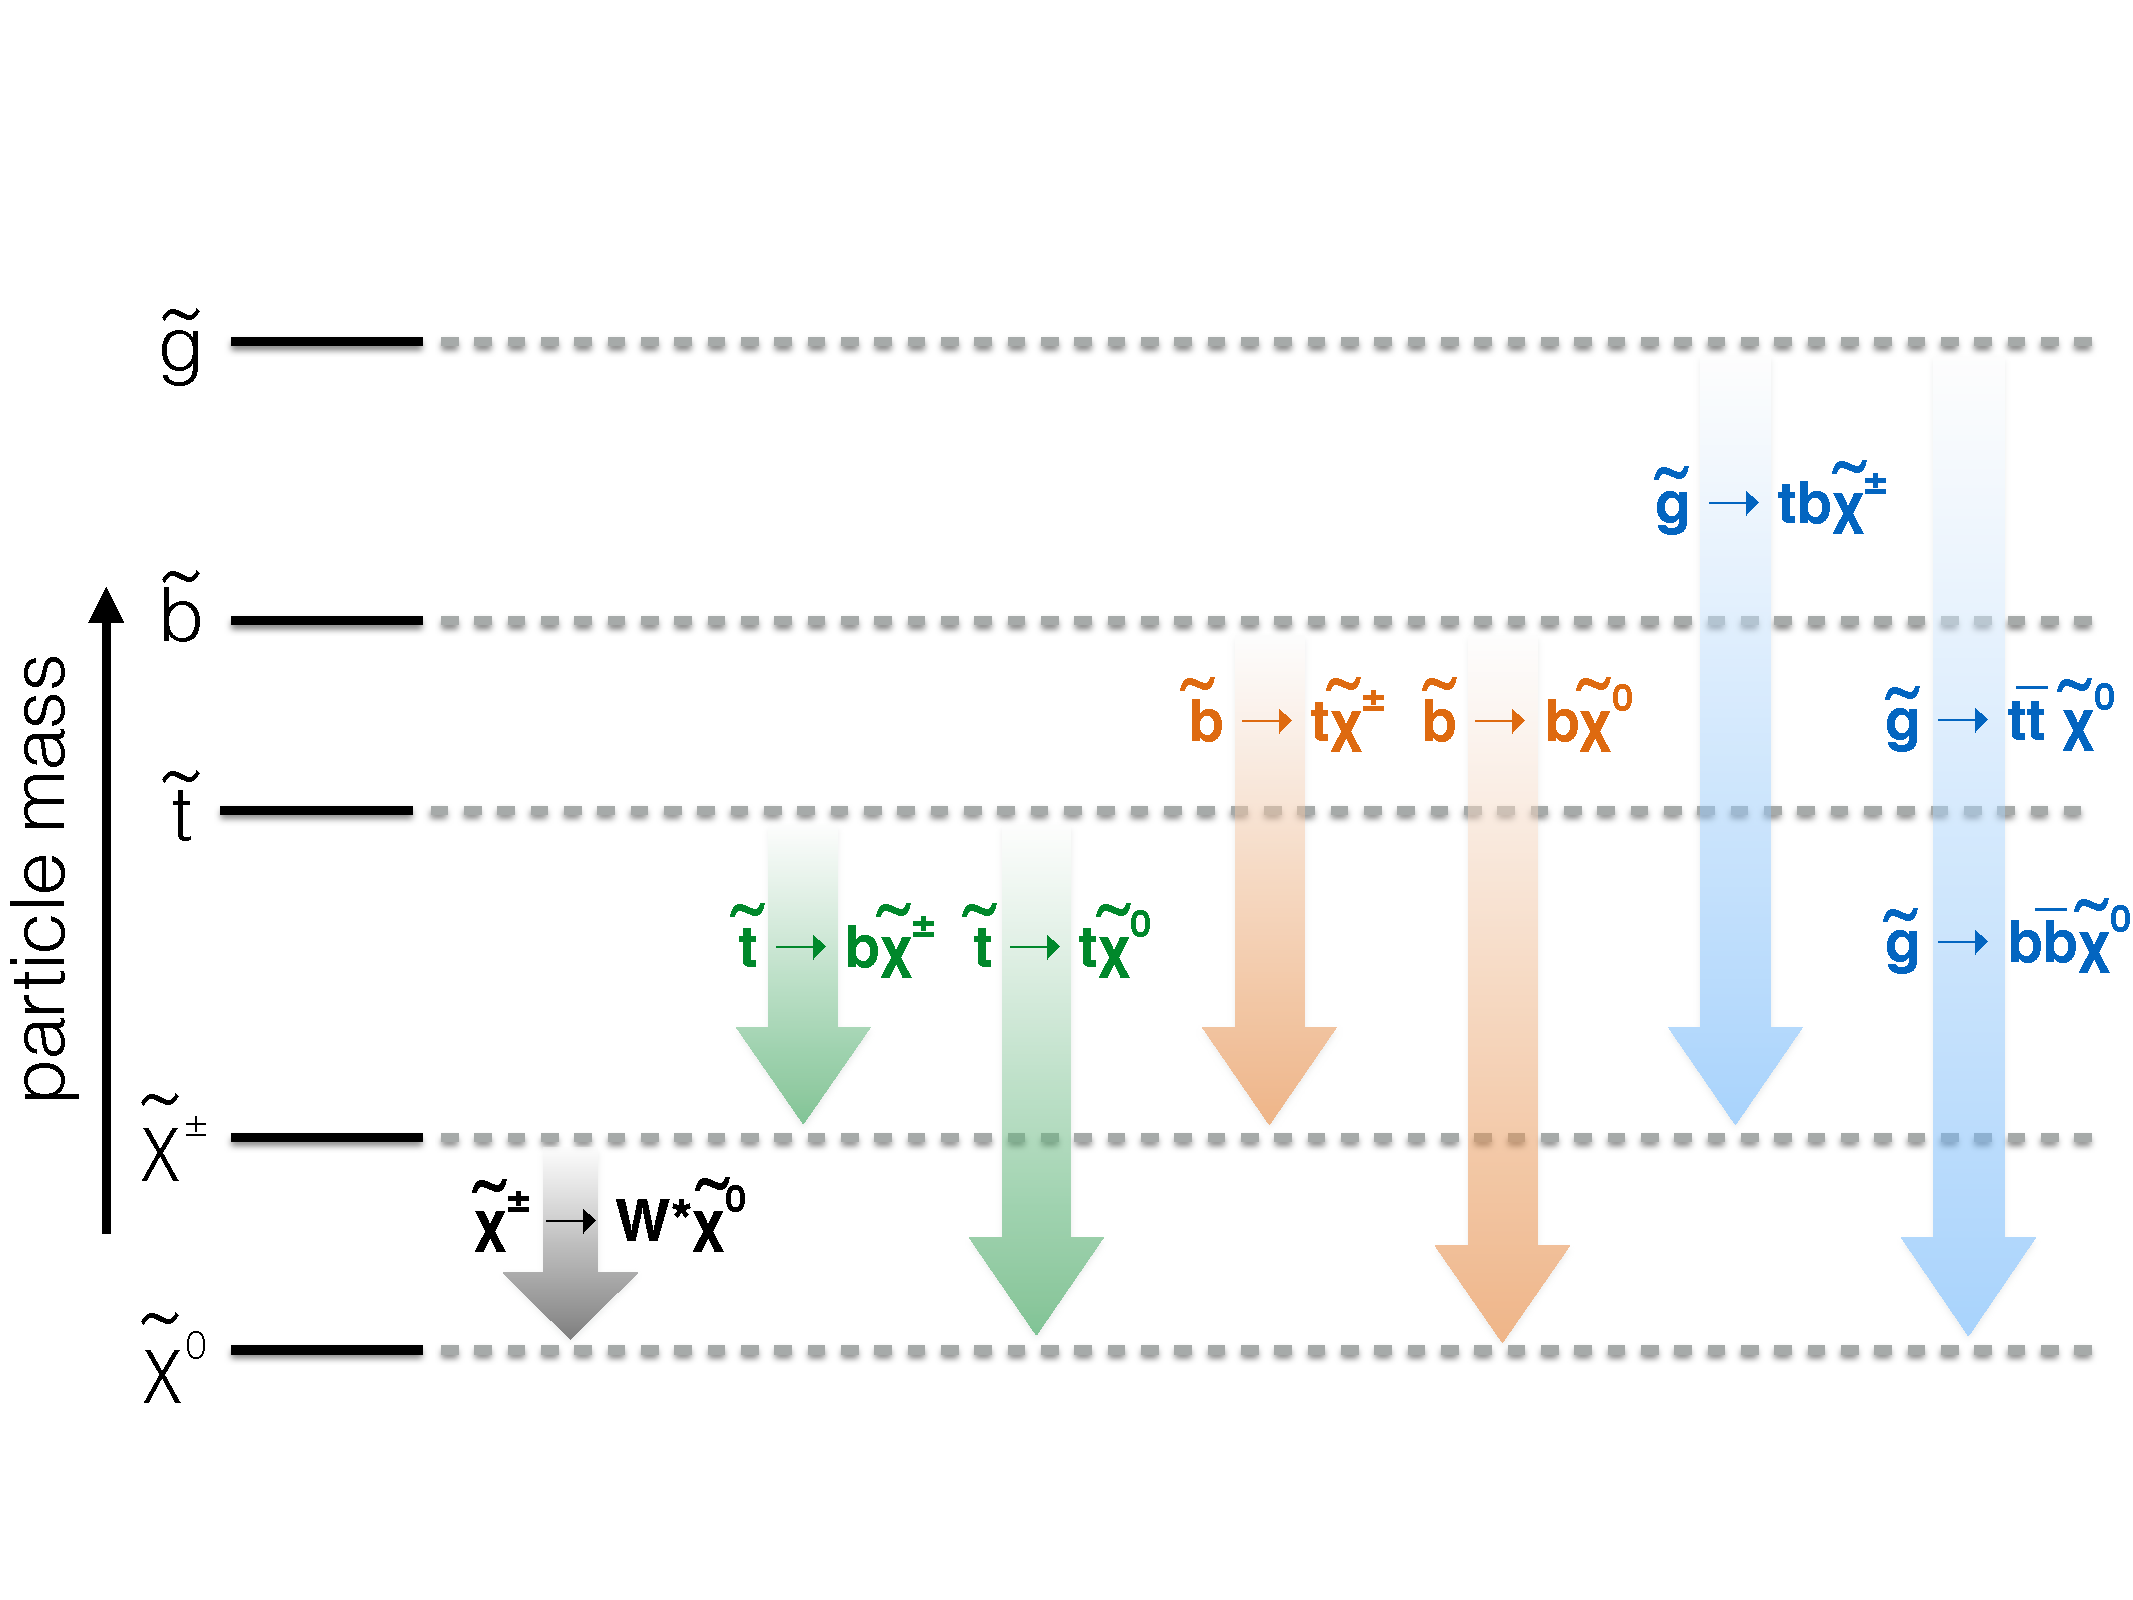
\includegraphics[width=0.85\textwidth]{figs/analysis8TeV/naturalSpectrum.pdf}
\caption{\label{fig:spectrum} The simplified natural SUSY spectrum
  considered in this paper, along with the assumed decay modes.}
\end{figure}

In Ch.~\ref{ch:analysis8TeV} and Ch.~\ref{ch:analysis13TeV}, natural simplified SUSY scenarios are used to interpret
results. The LSP is the lightest neutralino $\chiz_1$ while the NLSP
is the lightest chargino $\chipm_1$.  They are both higgsinos and
their mass splitting is taken to be 5\GeV. The NLSP decays to the LSP
and a virtual $\PW$ boson ($\chipm_1 \to \PW^{\ast} \chiz_1$). The
other SUSY particles accessible at the LHC are the gluino and the
lightest top and bottom squarks. All other SUSY particles are
assumed to be too heavy to participate in the interactions. The SUSY
particles and their possible decay modes within this natural SUSY
spectrum are summarized in Fig.~\ref{fig:spectrum}.

In the context of this natural spectrum, several simplified
models~\cite{ArkaniHamed:2007fw,Alwall:2008ag,Alwall:2008va,Alves:2011sq,Alves:2011wf,Graesser:2012qy}
are considered for gluino pair production, based on three-body gluino
decays, in which each gluino decays to one of the following final states~\cite{SUS-11-016}:
\begin{itemize}
\item a top quark (antiquark) and a bottom antiquark (quark),
  and the NLSP; 
\item a top quark-antiquark ($\ttbar$) pair and the LSP;
\item a bottom quark-antiquark ($\bbbar$) pair and the LSP.
\end{itemize}
Furthermore, we separately consider the case in which each gluino
decays to
\begin{itemize}
\item a first or second generation quark-antiquark ($\qqbar$) pair and the LSP.
\end{itemize}

\begin{figure*}[thb!]
\centering
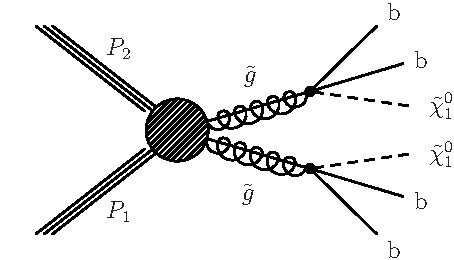
\includegraphics[width=0.32\textwidth]{figs/theory/T1bbbb.pdf}
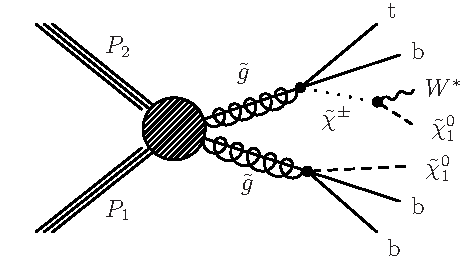
\includegraphics[width=0.32\textwidth]{figs/theory/T1tbbb.pdf}
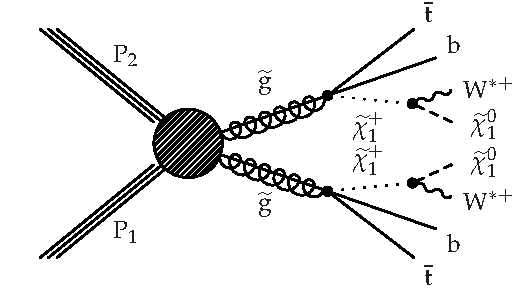
\includegraphics[width=0.32\textwidth]{figs/theory/T1ttbb.pdf} \\
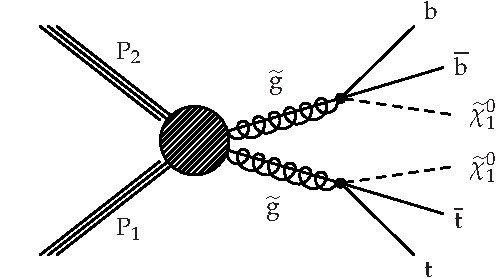
\includegraphics[width=0.32\textwidth]{figs/theory/T1tbtb.pdf} 
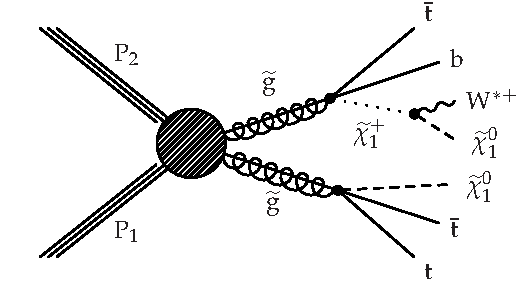
\includegraphics[width=0.32\textwidth]{figs/theory/T1tttb.pdf}
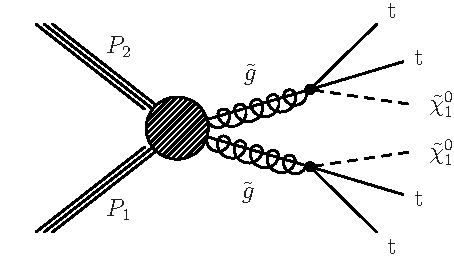
\includegraphics[width=0.32\textwidth]{figs/theory/T1tttt.pdf} \\
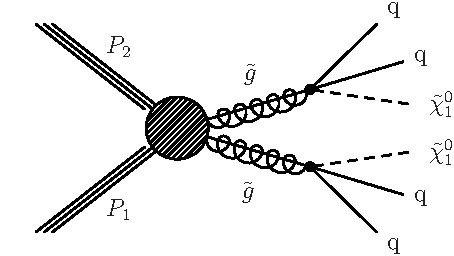
\includegraphics[width=0.32\textwidth]{figs/theory/T1qqqq.pdf} \\
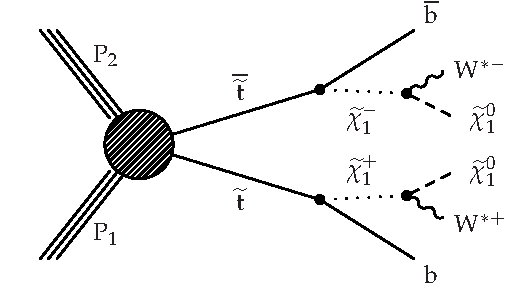
\includegraphics[width=0.32\textwidth]{figs/theory/T2bw.pdf}
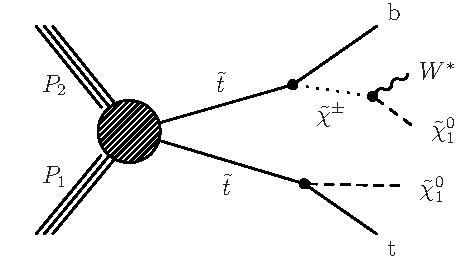
\includegraphics[width=0.32\textwidth]{figs/theory/T2tb.pdf}
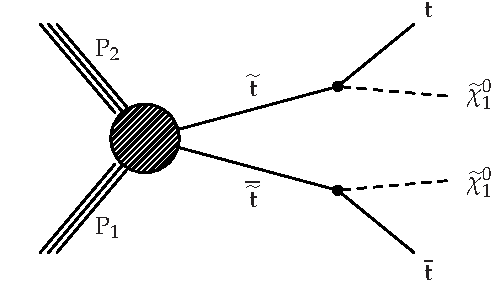
\includegraphics[width=0.32\textwidth]{figs/theory/T2tt.pdf}
\caption{Diagrams displaying the event topologies of gluino (upper 7
  diagrams) and top-squark (lower 3 diagrams) pair production
  considered in this thesis.\label{fig:SMSDiagrams}}
\end{figure*}

In addition, several simplified models are considered for
the production of top-squark pairs, in which each top squark decays to
one of the following final state:
 \begin{itemize}
\item a bottom quark and the NLSP;
\item a top quark and the LSP.
\end{itemize}

The corresponding Feynman diagrams are shown in
Fig.~\ref{fig:SMSDiagrams}.

\subsection{Technical Implentation in \PYTHIA}
To simplify the treatment of the sparticle decays in \PYTHIA v6.4.26, we directly implement three-body decays of
the form $\chipm_1 \to \chiz_1 f f^{\prime}$, with branching ratios
as shown in Table~\ref{tab:nlspbr}.
\begin{table}
\centering
\begin{tabular}{l|r}
decay mode & branching ratio \\\hline
$\chip_1 \to \chiz_1 u \bar d$ &  35.1\%\\
$\chip_1 \to \chiz_1 c \bar s$ &  35.1\%\\
$\chip_1 \to \chiz_1 e^+ \nu_e$ &  11.7\%\\
$\chip_1 \to \chiz_1 \mu^+ \nu_{\mu}$ &  11.7\%\\
$\chip_1 \to \chiz_1 \tau^+ \nu_{\tau}$ &  6.4\%
\end{tabular}
\caption{\label{tab:nlspbr}Table of branching ratios implemented in
  \PYTHIA v6.4.26 for the NLSP
  $\chipm_1$ in the simplified natural SUSY model considered in this chapter.}
\end{table}